%% See http://www.oxfordjournals.org/our_journals/bioinformatics/for_authors/general.html for author information

\documentclass{bioinfo}



\copyrightyear{2011}
\pubyear{2011}

\hyphenation{
be-tween
trans-late
i-den-ti-fiers
el-e-ments
path-way
con-tent
re-search-ers
in-di-vid-u-al
de-scrip-tion
path-way
i-den-ti-fi-ers
read-a-ble
microRNA
microRNAs
miRNA
miRNAs
straight-for-ward
}

\begin{document}
\application
\firstpage{1}


\title[InCroMAP]{InCroMAP: Integrated analysis of cross-platform microarray and pathway data}

\author[Wrzodek \textit{et~al}]{Clemens Wrzodek\,$^{1,*}$, Johannes Eichner\,$^{1}$ and Andreas Zell\,$^{1,}$\footnote{to whom correspondence should be addressed}}
\address{$^{1}$Center for Bioinformatics Tuebingen (ZBIT), University of Tuebingen, 72076 T\"ubingen, Germany}

\history{Received on XXXXX; revised on XXXXX; accepted on XXXXX}

\editor{Associate Editor: XXXXXXX}

\maketitle

\begin{abstract}

% TODO: Vor Submission Example DNAm data set checken ob sie noch sinn ergeben!
\section{Summary:}
%
Microarrays are commonly used to detect changes in gene expression between different biological samples. Therefore, many analysis tools are available that offer visualizations, statistical analysis and more sophisticated analysis methods. Most of those tools are designed specifically for messenger RNA microarrays. But today, more and more different microarray platforms are available. Changes in DNA methylation, MicroRNA expression or even protein phosphorylation states can be detected with specialized arrays. For these microarray technologies, the amount of available tools is very little, compared to mRNA analysis tools. Especially, a joint analysis of different microarray platforms that have been employed on the same set of biological samples is hardly supported by most microarray analysis tools.

We here present InCroMAP, a high-level microarray data analysis tools that can be used to perform single and integrated microarray data analysis. Currently, InCroMAP supports mRNA, microRNA, DNA methylation and protein modification datasets.
Several methods are offered that allow for an integrated analysis of those platforms.
% TODO: Satz �ber integrated
The available features of InCroMAP range from visualization of DNA methylation data, over annotation of microRNA targets and integrated gene set enrichment analysis to a joint visualization of all platforms in one pathway.



% Employing microarrays for the analysis of diverse biological samples has become
% Viele High-level microarray data analysis tools
% Die meisten fokus of mRNA
% deutlich weniger f�r miRNA, DNAm oder protein [mod.]
%
% Wir pr�sentieren InCroMAP, was h-level single dataset analysis kann, enrichments, visualisierung (DNAm), miRNA targets, pathway-visualisierung, uvm.
% Bridges the gap / "MAcht den Sprung" zu integrated analysis (pairing, multiple i., integr. enrichment, integr. pwb vis).
%
% High-level analysis tools for microarray data are

\section{Availability:}
InCroMAP is freely available as Java\texttrademark{} application at \href{http://www.cogsys.cs.uni-tuebingen.de/software/InCroMAP/}{www.cogsys.cs.uni-tuebingen.de/software/InCroMAP}.

% And a comprehensive documentation
%The described method is implemented as part of the InCroMAP application that is freely available at \href{http://www.cogsys.cs.uni-tuebingen.de/software/InCroMAP/}{www.cogsys.cs.uni-tuebingen.de/software/InCroMAP}.
%
%The described methods are implemented in InCroMAP, a tool for integrated analysis of cross-platform microarray and Pathway data.
%InCroMAP is a Java\texttrademark{} application that provides an interactive, user-friendly and easy-to-use graphical user interface (GUI), and is freely available under the LGPL version 3 license from \href{http://www.cogsys.cs.uni-tuebingen.de/software/InCroMAP/}{www.cogsys.cs.uni-tuebingen.de/software/InCroMAP}. The application can import all mentioned data types, is able to automatically download and layout KEGG pathways, and apply all described visualization methods on those pathways. The resulting graphs can be exported as JPG, GIF, TGF, GML or GraphML. Furthermore, many options are provided that control, e.g., the mapping of expression values to a continuous color gradient and allow for customization of the generated cross-platform pathway visualizations.

\section{Contact:} \href{mailto:clemens.wrzodek@uni-tuebingen.de}{clemens.wrzodek@uni-tuebingen.de}
\end{abstract}


\section{Introduction}
%
%Verschiedene Software Produkte:
%=================================
%Commercial vs. Non-Commercial (academic, open source)
%
%Ingenuity (mit PW, miRNA targets), more advanced
%Agilent Genespring (Herstelller eigene software)
%Genedata (Expressioniost)
%Chipster (auch ngs, protein, etc.)
%
%Mayday
%R Interface (MultiExperiment Viewer (MeV))
%
%... aber wir sind more sophisticated, bauen darauf auf. Eher Richtung ingenuity.
%
Typical workflows for the analysis of microarray data involve several steps. The procedures usually begin with the preparation of samples and arrays, followed by conduction of the experiments up to scanning the array in order to obtain the initial raw data in the computer. Depending on the actual array, several quality control and low-level data analysis steps are now performed \emph{in silico}. Common workflows mostly include normalization, annotation of gene identifiers and calculation of statistical comparison values (such as p-values, fold changes or log ratios). Most of these tasks are often performed in R, a statistical programming language (\href{http://www.r-project.org/}{www.r-project.org}), or derived applications with a graphical user interface (e.g., MultiExperiment Viewer -- \citealp{Saeed2006}, or Mayday -- \citealp{Dietzsch2006}). These two mentioned tools also bridge the gap to more sophisticated array analysis and visualization methods. But typically, the processed datasets can now be used in various high-level data analysis tools for further evaluation and data mining. A popular example is the commercial Ingenuity pathways analysis software (\href{http://www.ingenuity.com/}{www.ingenuity.com}), which links processed microarray datasets with pathway analysis.

But most of these high-level analysis tools are specialized on single platform analysis. Only a few approaches and very little tools are available for an integrated analysis of high-throughput data from heterogenous platforms.
%One of these examples is MMIA \citep{Nam2009}, a webtool that integrates microRNA and mRNA data.
Furthermore, not many software tools are freely available that offer suitable and easy-to-use analysis and visualization techniques for microarray platforms, other than mRNA expression.

Therefore, we developed InCroMAP, an easy-to-use and interactive application with a graphical user interface that is specialized on an integrated analysis of cross-platform microarray and pathway data. InCroMAP supports DNA methylation, messenger RNA, microRNA and protein modification datasets. Besides these platforms, it is possible to import any platform that contains expression values that can somehow be assigned to genes.
A special emphasis has been put on the usability of the application, hence all required files, e.g., for mapping gene identifiers to gene symbols, annotating mRNA targets to micoRNAs or pathways to visualize are either directly included in the application or downloaded dynamically in the background.


%Keine alternative (kein fold-change berechnen, Clustering, MA plot) sondern erg�nzend und darauf aufbauende analysen, insbesondere f�r integrated.

%%%%%%%%%%%%%%%%%%%%%  FIGURE  %%%%%%%%%%%%%%%%%%%%%%%%%%%%%%
\begin{figure*}[t]%figure1
\centerline{
  \noindent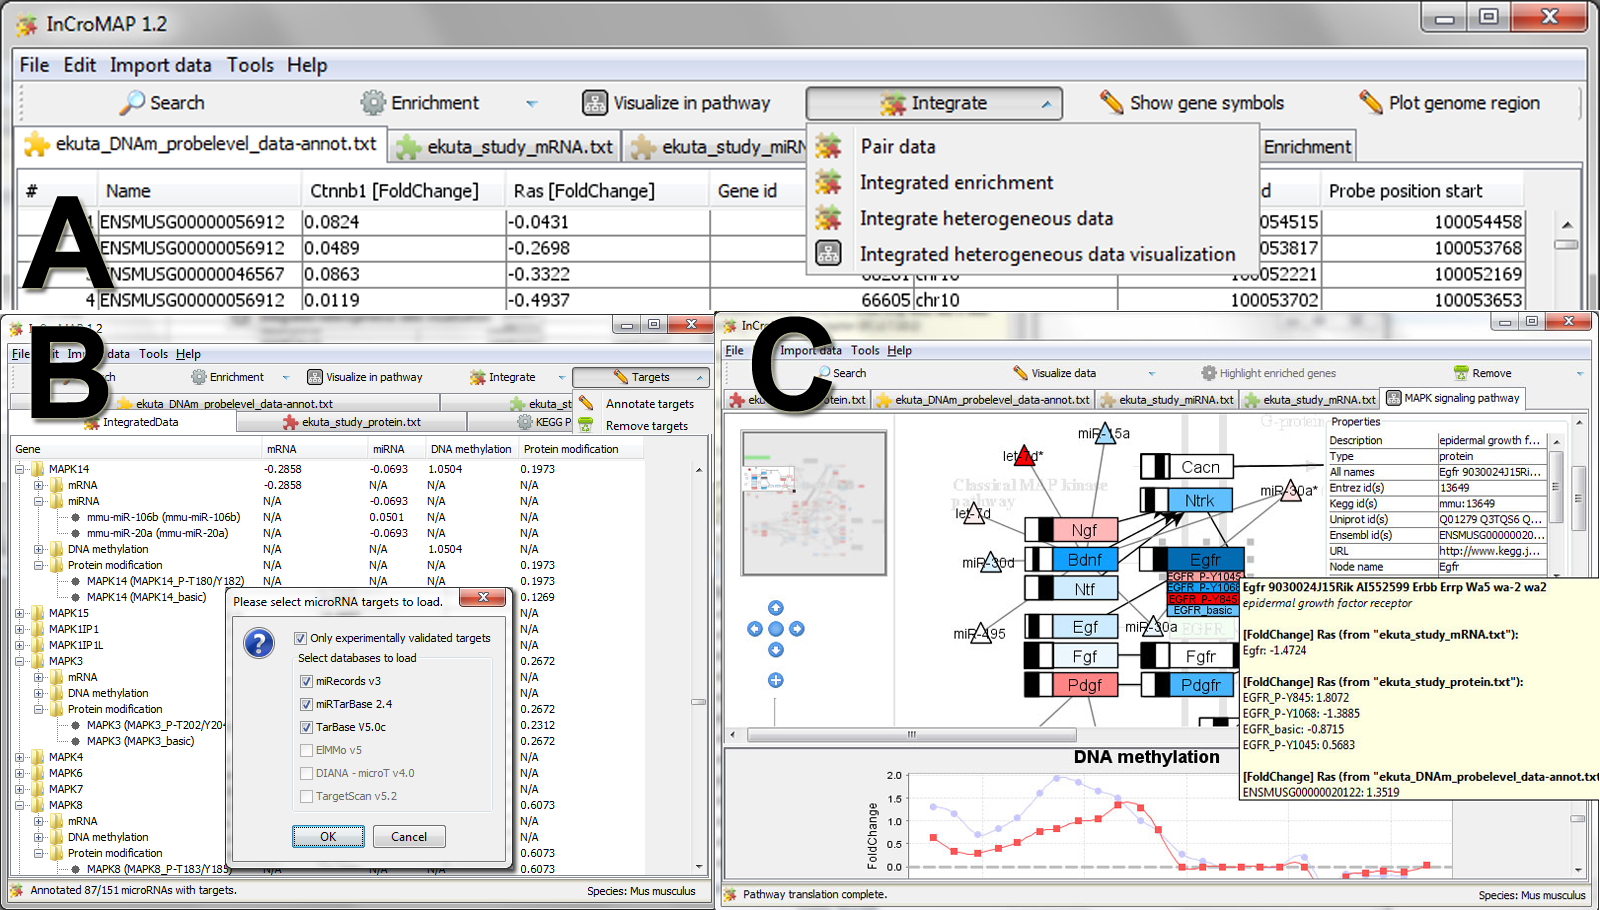
\includegraphics[width=\textwidth]{figures/Figure.png}
}
\caption{
Different views of InCroMAP. A) the popup menu shows different methods that are provided for a joint analysis of heterogeneous microarray platforms. B) MicroRNA datasets can be annotated with three experimental and three predicted miRNA target databases directly from within the application. In the background the result of the `integrate heterogeneous data' procedure is shown. C) Integrated pathway-based visualization of heterogenous microarray datasets allows to visualize up to four different platforms in a single pathway (excerpt from the `MAPK signaling' pathway). Pathway nodes can be selected to get more detailed information, including various plots for all assigned expression values from every platform (DNA methylation in the promoter region of \emph{Egfr} is depicted in the bottom part of C).
}\label{fig:01}
\end{figure*}
%%%%%%%%%%%%%%%%%%%%%%%%%%%%%%%%%%%%%%%%%%%%%%%%%%%%%%%%%%%%%


\begin{methods}
\section{Results}
\subsection{Integration of heterogeneous platforms}
To integrated data from multiple platforms, a common denominator must be established. The vast majority of all data is somehow associated to genes hence, integration of multiple data types is performed by mapping each probe to a gene. This procedure is straightforward for protein or mRNA datasets. DNA methylation datasets are region-based and can be mapped on genes by defining a window upstream and downstream of each gene's transcription start site. InCroMAP proposes a window of $-2,000$ and $+500$\,bps as default region, but users may change these values. Commonly, mRNA and protein data consists of protein coding genes and the relation between DNA methylation and mRNA is of regulatory nature. Therefore, integration of microRNA data is performed by annotating the genes of the mRNA targets to each microRNA. For this task, the user can choose between three microRNA target databases that contain experimentally verified targets and three databases with predicted targets \citep[databases reviewed in][]{Alexiou2009}.

%\subsection{Single dataset analysis}
%Even though the focus of InCroMAP is providing integrated analysis and visualization tools for cross-platform datasets, some single dataset analysis functionality is provided. This is important to verify hypotheses gained from integrated analysis or to compare integrated data analysis with single dataset analysis results. Single dataset features include gene set enrichment analysis (fast version with hypergeometric test as described, e.g., in \citealp{Backes2007}), using gene sets from the KEGG PATHWAY database, Gene Ontology and any gene set from the molecular signatures database \citep{Subramanian2005}. Gene set enrichment analysis on mRNA or protein datasets is straightforward, but implementations that can also handle DNA methylation or microRNA data are less common. Following the common pathway enrichment analysis, each dataset can be visualized separately in a pathway.
%Furthermore, potential mRNA targets of each microRNA can be inspected and DNA methylation data can be visualized within a given genomic location.


\subsection{Integrated data analysis}
A first approach to integratively investigate data from any two platforms is the `data pairing' procedure. This procedure shows two datasets next to each other hence, simplifying common lookup task such as investigating the effect of a differentially regulated mRNA on protein level. Further, this view is especially suitable to inspect the effect of microRNA expression on target mRNAs.
%Therefore, some additional columns are placed between the datasets that display the database in which this relation is specified or that allow for calculations of differences.
%F�r miRNA gut, AbsoluteSum kann berechnet werden um jede zu bekommen welche in protein und mRNA hochreguliert sind.
An arbitrary amount of platforms can be inspected, using the `integrate heterogenous data' procedure. To keep the clarity, only the most relevant information, i.e., the expression values (as fold changes or p-values) are shown. Therefore, one row is created for each gene and one column for each platform. This procedure requires mostly summarization of multiple values, which user's can control by picking mean, median, maximum, etc. A special representation is provided that integrated a tree in a table to allow expanding the node of each gene to show all platforms with associated values. If these are expanded more detailed information, such as the single probes or microRNAs targeting this gene's mRNA is displayed.
%
A popular method for a generic analysis of expression data is performing a gene set enrichment. We have extended this procedure to an integrated gene set enrichment that is able to perform enrichments across multiple platforms. The user can choose the datasets and thresholds for each dataset to calculate a p-value, using a hypergeometric test for each predefined gene set (see \citealp{Backes2007} for more information). InCroMAP supports gene sets from the KEGG PATHWAY database, Gene Ontology and any gene set from the molecular signatures database
(\href{http://www.broadinstitute.org/gsea/msigdb/}{www.broadinstitute.org/gsea/msigdb/}).
% Including the citation takes too much space... \citep{Subramanian2005}.
%

Visualization of expression data in pathways is supported for each single platform. Furthermore, InCroMAP allows for integratively visualizing data from all platforms in a single pathway. Therefore, node color is changed according to mRNA expression and small boxes are added and colored according to each protein modification's expression value. MicroRNAs are added as small colored triangles to the graph and connected to their targets with novel edges. DNA methylation data is indicated with a black bar that shows the maximum differential peak in each gene's promoter (stretching from the middle to the left to indicate hypomethylation and to the right for hypermethylation). This is an interactive graph, therefore allowing users to modify the layout and selecting nodes to get more detailed information and plots about all associated expression values.
%

Besides those integrated analysis methods, InCroMAP allows plotting region-based DNA methylation data in a genome plot with boxes for gene bodies, which in turn can be colored, e.g., according to mRNA expression. Further, all enrichments can also be performed on any single dataset, which is straightforward for mRNA or protein datasets, but implementations that can also handle DNA methylation or microRNA data are less common.


%Multiple Integration f�r mehrere, hierbei infos auf wunsch erst aufklappen.
%Integrated Enrichment
%PW-based visualization
%DNAm-region + mRNA f�rbung unten

\end{methods}
%\section{Conclusion}




\section*{Acknowledgement}
We gratefully acknowledge contributions from Andreas Dr\"ager and Finja B\"uchel, as well as the
whole MARCAR consortium.

\paragraph{Funding\textcolon} The research leading to these results has received funding from the Innovative Medicine Initiative Joint Undertaking (IMI JU) under grant agreement nr. 115001 (MARCAR project).
%This work was supported by the Innovative Medicine Initiative Joint Undertaking (IMI JU), MARCAR project [grant number 115001].


\paragraph{Conflict of Interest\textcolon} none declared.
%\vspace{-.1cm}


\bibliographystyle{natbib}

%XXX: Uncomment for dynamic reference addition
\bibliography{InCroMAP_appNote}




\end{document}
